%% beamer/knitr slides 
%% for Statistical Modeling and Data Visualization course @ UMass
%% Nicholas Reich: nick [at] schoolph.umass.edu


\documentclass[table]{beamer}\usepackage[]{graphicx}\usepackage[]{color}
%% maxwidth is the original width if it is less than linewidth
%% otherwise use linewidth (to make sure the graphics do not exceed the margin)
\makeatletter
\def\maxwidth{ %
  \ifdim\Gin@nat@width>\linewidth
    \linewidth
  \else
    \Gin@nat@width
  \fi
}
\makeatother

\definecolor{fgcolor}{rgb}{0.345, 0.345, 0.345}
\newcommand{\hlnum}[1]{\textcolor[rgb]{0.686,0.059,0.569}{#1}}%
\newcommand{\hlstr}[1]{\textcolor[rgb]{0.192,0.494,0.8}{#1}}%
\newcommand{\hlcom}[1]{\textcolor[rgb]{0.678,0.584,0.686}{\textit{#1}}}%
\newcommand{\hlopt}[1]{\textcolor[rgb]{0,0,0}{#1}}%
\newcommand{\hlstd}[1]{\textcolor[rgb]{0.345,0.345,0.345}{#1}}%
\newcommand{\hlkwa}[1]{\textcolor[rgb]{0.161,0.373,0.58}{\textbf{#1}}}%
\newcommand{\hlkwb}[1]{\textcolor[rgb]{0.69,0.353,0.396}{#1}}%
\newcommand{\hlkwc}[1]{\textcolor[rgb]{0.333,0.667,0.333}{#1}}%
\newcommand{\hlkwd}[1]{\textcolor[rgb]{0.737,0.353,0.396}{\textbf{#1}}}%
\let\hlipl\hlkwb

\usepackage{framed}
\makeatletter
\newenvironment{kframe}{%
 \def\at@end@of@kframe{}%
 \ifinner\ifhmode%
  \def\at@end@of@kframe{\end{minipage}}%
  \begin{minipage}{\columnwidth}%
 \fi\fi%
 \def\FrameCommand##1{\hskip\@totalleftmargin \hskip-\fboxsep
 \colorbox{shadecolor}{##1}\hskip-\fboxsep
     % There is no \\@totalrightmargin, so:
     \hskip-\linewidth \hskip-\@totalleftmargin \hskip\columnwidth}%
 \MakeFramed {\advance\hsize-\width
   \@totalleftmargin\z@ \linewidth\hsize
   \@setminipage}}%
 {\par\unskip\endMakeFramed%
 \at@end@of@kframe}
\makeatother

\definecolor{shadecolor}{rgb}{.97, .97, .97}
\definecolor{messagecolor}{rgb}{0, 0, 0}
\definecolor{warningcolor}{rgb}{1, 0, 1}
\definecolor{errorcolor}{rgb}{1, 0, 0}
\newenvironment{knitrout}{}{} % an empty environment to be redefined in TeX

\usepackage{alltt}


%       ************************************************
%       **        LaTeX preamble to be used with all 
%	**        statsTeachR labs/handouts.
%
%	Author: Nicholas G Reich
%	Last modified: 14 January 2014
%	************************************************

% \documentclass[table]{beamer}

%	Set theme (a nice plain one)
\usetheme{Malmoe}

%	Use named colors, set main color of theme
%		to match Web site color:
\definecolor{MainColor}{RGB}{10, 74, 109}
\colorlet{MainColorMedium}{MainColor!50}
\colorlet{MainColorLight}{MainColor!20}
\usecolortheme[named=MainColor]{structure} 

%	For tables
%[dvipsnames] [table]
\usepackage{xcolor}

%% calling tabu.sty, assuming a particular directory structure
\usepackage{../../slide-includes/tabu}	% Even fancier than tabulary
\usepackage{multirow}

%	Just for the degree symbol
\usepackage{textcomp}

%	Get rid of footline (page, author, etc. on each slide)
\setbeamertemplate{footline}{}
%	Get rid of navigation buttons
\setbeamertemplate{navigation symbols}{}

%	Make footnotes not ugly
\usepackage{hanging}
\setbeamertemplate{footnote}{\raggedright\hangpara{1em}{1}\makebox[1em][l]{\insertfootnotemark}\footnotesize\insertfootnotetext\par}

%	Text style for code snippets inline in text:
\newcommand{\codeInline}[1]{\texttt{#1}}

%	Text style for emphasis stronger than \emph:
%		(Note, this doesn't toggle the way \emph does.
%			(Note, this can be done, didn't seem worth the trouble.))
\newcommand{\strong}[1]{{\bfseries{#1}}}


%        ******	Define title page	**********************
\setbeamertemplate{title page}{
	{\color{MainColor}
	% There must be a better way than this -vspace at
	%	 the top and bottom of the page to reduce the 
	%	 bottom margin, but I can't find one that works.
	\vspace{-6em}

% 	% Go to a lot of trouble to get the title in a
% 	%	nice box, since customizing a beamer block
% 	%	does not entirely work here (I don't know why)
	\newlength{\titleBoxWidth}
	\setlength{\titleBoxWidth}{\textwidth}
	\addtolength{\titleBoxWidth}{-2.0em}
	\setlength{\fboxsep}{1.0em}
	\setlength{\fboxrule}{0pt}
	\fcolorbox{MainColor!25}{MainColor!25}{
		\parbox{\titleBoxWidth}{
			\raggedright
			\LARGE\textbf{\inserttitle}
		}	% end parbox
	}	% end fcolorbox

	\vfill
	\small{Author: \insertauthor}
	\vspace{\baselineskip}

	\small{\Course}

	\small{\Instructor}
	\vspace{\baselineskip}

	%\small{\emph{This material is part of the \strong{statsTeachR} project}}

	\vspace{0.33\baselineskip}\scriptsize{\emph{\LicenseText}}


		\vspace{-15em}

	}	% end color
	\clearpage
}	% end define title page

%	The following variables are assumed by the standard preamble:
%	Global variable containing module name:
\title{Introduction to \\ Telling Stories with Data}
%	Global variable containing module shortname:
%		(Currently unused, may be used in future.)
\newcommand{\ModuleShortname}{introRegression}
%	Global variable containing author name:
\author{Nicholas G Reich}
%	Global variable containing text of license terms:
\newcommand{\LicenseText}{Made available under the Creative Commons Attribution-ShareAlike 3.0 Unported License: http://creativecommons.org/licenses/by-sa/3.0/deed.en\textunderscore US }
%	Instructor: optional, can leave blank.
%		Recommended format: {Instructor: Jane Doe}
\newcommand{\Instructor}{}
%	Course: optional, can leave blank.
%		Recommended format: {Course: Biostatistics 101}
\newcommand{\Course}{}


\input{../../slide-includes/shortcuts}

\hypersetup{colorlinks,linkcolor=,urlcolor=MainColor}


%	******	Document body begins here	**********************
\IfFileExists{upquote.sty}{\usepackage{upquote}}{}
\begin{document}

%	Title page
\begin{frame}[plain]
	\titlepage
\end{frame}

%	******	Everything through the above line must be placed at
%		the top of any TeX file using the statsTeachR standard
%		beamer preamble. 






%%%%%%%%%%%%%%%%%%%%%%%%%%%%%%%%%%%%%%%%%%

\begin{frame}[fragile]{State-level SAT score data (1994-95)}

\begin{knitrout}
\definecolor{shadecolor}{rgb}{0.969, 0.969, 0.969}\color{fgcolor}
\includegraphics[width=\maxwidth]{figure/sat1-1} 

\end{knitrout}


\end{frame}



%%%%%%%%%%%%%%%%%%%%%%%%%%%%%%%%%%%%%%%%%%


\begin{frame}[fragile]{State-level SAT score data (1994-95)}

\begin{knitrout}
\definecolor{shadecolor}{rgb}{0.969, 0.969, 0.969}\color{fgcolor}
\includegraphics[width=\maxwidth]{figure/sat1a-1} 

\end{knitrout}


\end{frame}

%%%%%%%%%%%%%%%%%%%%%%%%%%%%%%%%%%%%%%%%%%



\begin{frame}[fragile]{State-level SAT score data (1994-95)}

\begin{knitrout}
\definecolor{shadecolor}{rgb}{0.969, 0.969, 0.969}\color{fgcolor}
\includegraphics[width=\maxwidth]{figure/sat2-1} 

\end{knitrout}


\end{frame}


%%%%%%%%%%%%%%%%%%%%%%%%%%%%%%%%%%%%%%%%%%

\begin{frame}{The SAT example}

\begin{block}{What is the outcome variable?}
\vskip3em
\end{block}

\begin{block}{What is the covariate or predictor variable?}
\vskip3em
\end{block}

\begin{block}{What other data might be part of this story?}
\vskip3em
\end{block}


\end{frame}

%%%%%%%%%%%%%%%%%%%%%%%%%%%%%%%%%%%%%%%%%%



\begin{frame}[fragile]{State-level SAT score data (1994-95)}

\begin{knitrout}
\definecolor{shadecolor}{rgb}{0.969, 0.969, 0.969}\color{fgcolor}
\includegraphics[width=\maxwidth]{figure/sat3-1} 

\end{knitrout}


\end{frame}

%%%%%%%%%%%%%%%%%%%%%%%%%%%%%%%%%%%%%%%%%%

\begin{frame}[fragile]{State-level SAT score data (1994-95)}

\begin{knitrout}
\definecolor{shadecolor}{rgb}{0.969, 0.969, 0.969}\color{fgcolor}
\includegraphics[width=\maxwidth]{figure/sat4-1} 

\end{knitrout}

\end{frame}



%%%%%%%%%%%%%%%%%%%%%%%%%%%%%%%%%%%%%%%%%%

\begin{frame}[fragile]{State-level SAT score data (1994-95)}

\begin{knitrout}
\definecolor{shadecolor}{rgb}{0.969, 0.969, 0.969}\color{fgcolor}
\includegraphics[width=\maxwidth]{figure/sat4a-1} 

\end{knitrout}

\end{frame}


%%%%%%%%%%%%%%%%%%%%%%%%%%%%%%%%%%%%%%%%%%

\begin{frame}[fragile]{State-level SAT score data (1994-95)}

\begin{knitrout}
\definecolor{shadecolor}{rgb}{0.969, 0.969, 0.969}\color{fgcolor}
\includegraphics[width=\maxwidth]{figure/sat5-1} 

\end{knitrout}

\end{frame}


%%%%%%%%%%%%%%%%%%%%%%%%%%%%%%%%%%%%%%%%%%

\begin{frame}[fragile]{State-level SAT score data (1994-95)}

\begin{knitrout}
\definecolor{shadecolor}{rgb}{0.969, 0.969, 0.969}\color{fgcolor}
\includegraphics[width=\maxwidth]{figure/sat6-1} 

\end{knitrout}

\end{frame}



%%%%%%%%%%%%%%%%%%%%%%%%%%%%%%%%%%%%%%%%%%

\begin{frame}[fragile]{State-level SAT score data (1994-95)}

\begin{knitrout}
\definecolor{shadecolor}{rgb}{0.969, 0.969, 0.969}\color{fgcolor}
\includegraphics[width=\maxwidth]{figure/sat7-1} 

\end{knitrout}

\end{frame}



%%%%%%%%%%%%%%%%%%%%%%%%%%%%%%%%%%%%%%%%%%

\begin{frame}[fragile]{State-level SAT score data (1994-95)}

What can we conclude from all of this? (BTW, this is an example of \href{http://en.wikipedia.org/wiki/Simpson%27s_paradox}{"Simpson's Paradox"}.)

\end{frame}


%%%%%%%%%%%%%%%%%%%%%%%%%%%%%%%%%%%%%%%%%%

\begin{frame}{Regression modeling}

The process of using data to describe the relationship between outcomes and predictors is called modeling.
\bi
	\myitem Models are models, not reality.
	\myitem ``All models are wrong, but some are useful."
	\myitem Introduce structure to our model that balances realism with ``goodness of fit''. \ei

\end{frame}


%%%%%%%%%%%%%%%%%%%%%%%%%%%%%%%%%%%%%%%%%%

\begin{frame}{Things to come}

\includegraphics[width=\textwidth]{../../slide-includes/data-science-program.png}

\end{frame}

%%%%%%%%%%%%%%%%%%%%%%%%%%%%%%%%%%%%%%%%%%

\begin{frame}[fragile]{Beware of correlation!}

\begin{figure}[t]
    \includegraphics[width=\textwidth]{us-spending-on-science-space-and-technology_suicides-by-hanging-strangulation-and-suffocation}  
\end{figure}

\end{frame}

\begin{frame}[fragile]{Beware of correlation!}

\begin{figure}[t]
    \includegraphics[width=\textwidth]{number-people-who-drowned-by-falling-into-a-swimming-pool_number-of-films-niclas-cage-appeared-in}  
\end{figure}

\footnotesize{Hat tip to \href{http://www.tylervigen.com}{www.tylervigen.com}}
\end{frame}



\begin{frame}[fragile]

\begin{figure}[t]
    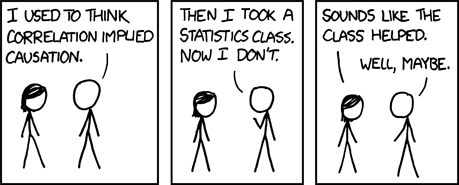
\includegraphics[width=\textwidth]{figure-static/correlation.png}  
\end{figure}

\footnotesize{https://xkcd.com/552/}
\end{frame}



%%%%%%%%%%%%%%%%%%%%%%%%%%%%%%%%%%%%%%%%%%

\begin{frame}[fragile]{Appendix: Code for plotting}

\scriptsize
\begin{knitrout}
\definecolor{shadecolor}{rgb}{0.969, 0.969, 0.969}\color{fgcolor}\begin{kframe}
\begin{alltt}
\hlkwd{library}\hlstd{(mosaicData)}
\hlkwd{library}\hlstd{(ggplot2)}
\hlkwd{theme_set}\hlstd{(}\hlkwd{theme_bw}\hlstd{())}
\hlkwd{data}\hlstd{(SAT)}
\hlstd{SAT}\hlopt{$}\hlstd{fracgrp} \hlkwb{=} \hlkwd{cut}\hlstd{(SAT}\hlopt{$}\hlstd{frac,} \hlkwc{breaks}\hlstd{=}\hlkwd{c}\hlstd{(}\hlnum{0}\hlstd{,} \hlnum{22}\hlstd{,} \hlnum{49}\hlstd{,} \hlnum{81}\hlstd{),}
                  \hlkwc{labels}\hlstd{=}\hlkwd{c}\hlstd{(}\hlstr{"low"}\hlstd{,} \hlstr{"medium"}\hlstd{,} \hlstr{"high"}\hlstd{))}
\hlkwd{ggplot}\hlstd{(SAT)} \hlopt{+}
    \hlkwd{geom_text}\hlstd{(}\hlkwd{aes}\hlstd{(}\hlkwc{x}\hlstd{=salary,} \hlkwc{y}\hlstd{=sat,} \hlkwc{label}\hlstd{=state),} \hlkwc{size}\hlstd{=}\hlnum{4}\hlstd{,} \hlkwc{show.legend}\hlstd{=}\hlnum{FALSE}\hlstd{)} \hlopt{+}
    \hlkwd{xlab}\hlstd{(}\hlstr{"est. average public school teacher salary"}\hlstd{)} \hlopt{+}
    \hlkwd{ylab}\hlstd{(}\hlstr{"average total SAT score"}\hlstd{)}
\end{alltt}
\end{kframe}
\end{knitrout}

More plotting code available \href{https://github.com/nickreich/data-stories/blob/gh-pages/assets/lectures/lecture1-intro-regression/lecture1-intro-regression.Rnw#L254}{here}.

\end{frame}

\end{document}
